% Szglab4
% ===========================================================================
%
\chapter{Prototípus koncepciója}

\thispagestyle{fancy}
\setcounter{section}{0}
\section{Változások a specifikációban}

\subsection{Köd}
\textbf{A tornyokra időnként köd ereszkedik, aminek következtében a látás erősen lecsökken. Ez hatással van a lövésre.}\\
Egy új Fog osztályt vezetünk be. Ennek van egy darab statikus getRangeMultiplier() metódusa, ami visszaadja mennyivel csökkenjen a látótáv, valamint van egy setFog(bool), amivel be lehet állítani, hogy van-e köd vagy nincs. Ha nincs köd beállítva getRangeMultiplier() 1-et ad vissza.

\subsection{Elágazások}
\textbf{A játékosok által járható útvonalon lehetnek elágazások és becsatlakozások. Az elágazásokon az egyes játékosok véletlenszerűen mennek a különböző irányokba.}\\
Mi a feladatot alapból így specifikáltuk, ezért változásra nincs szükség.
\subsection{Új lövedék}
\textbf{A tornyokban elvétve lehetnek olyan lövedékek, amelyek az eltalált játékost kettőbe vágják. A két játékos egymástól függetlenül él tovább, csökkentett életerővel.}\\
Ehhez létrehoztunk egy új SplitterProjectile osztályt, ami a Projectile osztályból származik le. Valamint hozzáadtunk az Enemy osztályhoz egy split() metódust. A Game osztályhoz pedig egy addEnemy(Enemy) metódust adtunk, amit a SplitterProjectile hív meg egy callback-el, amikor kettévágta az ellenséget.

\subsection{Módosult osztálydiagram}
\begin{figure}[H]
\begin{center}
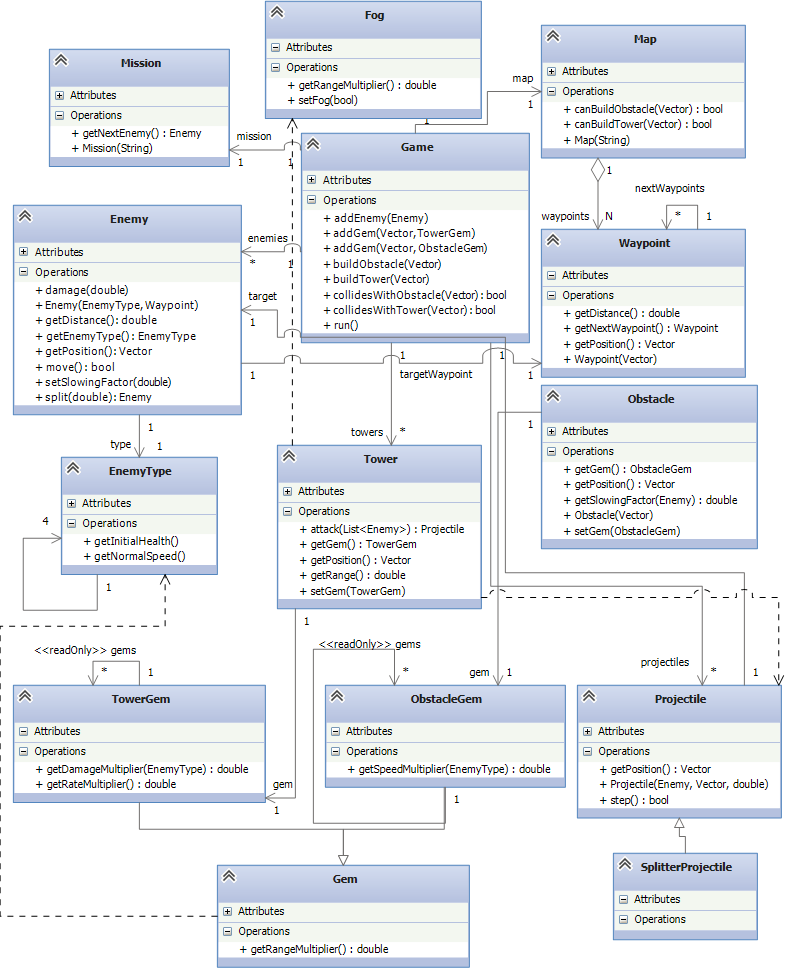
\includegraphics[width=17cm]{images/ch07/class_new.png}
\caption{Osztály diagram}
\label{fig:classDiagNew}
\end{center}
\end{figure}

\subsection{Módosult szekvencia diagramok}
\begin{figure}[H]
\begin{center}
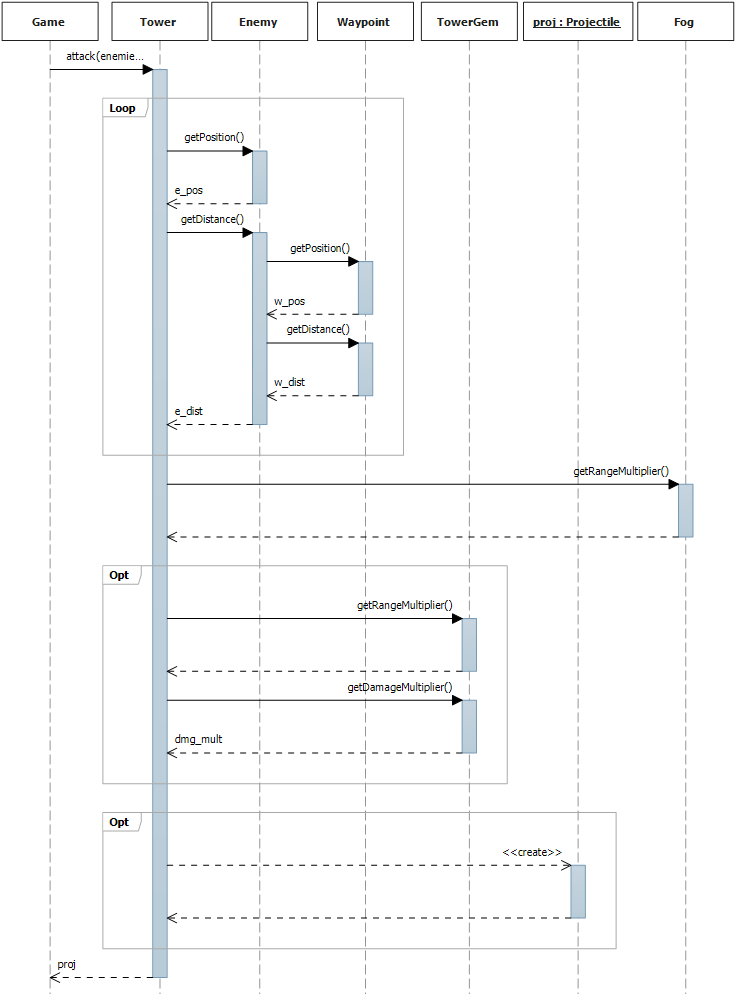
\includegraphics[width=17cm]{images/ch07/attack_enemy.png}
\caption{Ellenség támadása}
\label{fig:enemyAttackNew}
\end{center}
\end{figure}

\begin{figure}[H]
\begin{center}
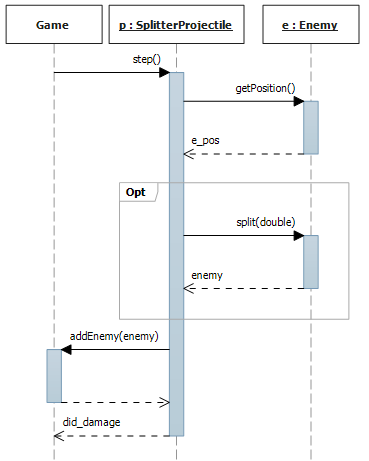
\includegraphics[width=10cm]{images/ch07/splitterprojectile_step.png}
\caption{Újfajta lövedék mozgatása}
\label{fig:splitProjMove}
\end{center}
\end{figure}


\section{Prototípus interface-definíciója}
\comment{Definiálni kell a teszteket leíró nyelvet. Külön figyelmet kell fordítani arra, hogy ha a rendszer véletlen elemeket is tartalmaz, akkor a véletlenszerűség ki-bekapcsolható legyen, és a program determinisztikusan is tesztelhető legyen.}

\subsection{Az interfész általános leírása}
\comment{A protó (karakteres) input és output felületeit úgy kell kialakítani, hogy az input fájlból is vehető legyen illetőleg az output fájlba menthető legyen, vagyis kommunikációra csak a szabványos be- és kimenet használható.}

\subsection{Bemeneti nyelv}
\comment{Definiálni kell a teszteket leíró nyelvet. Külön figyelmet kell fordítani arra, hogy ha a rendszer véletlen elemeket is tartalmaz, akkor a véletlenszerűség ki-bekapcsolható legyen, és a program determinisztikusan is futtatható legyen. A szálkezelést is tesztelhető, irányítható módon kell megoldani.}

\begin{itemize}
\item Parancs1
	\begin{itemize}
	\item Leírás:
	\item Opciók:
	\end{itemize}
\item Parancs2
	\begin{itemize}
	\item Leírás:
	\item Opciók:
	\end{itemize}

\end{itemize}

\comment{Ha szükséges, meg kell adni a konfigurációs (pl. pályaképet megadó) fájlok nyelvtanát is.}

\subsection{Kimeneti nyelv}
\comment{Egyértelműen definiálni kell, hogy az egyes bemeneti parancsok végrehajtása után előálló állapot milyen formában jelenik meg a szabványos kimeneten.}

\section{Összes részletes use-case}
\comment{A use-case-eknek a részletezettsége feleljen meg a kezelői felületnek, azaz a felület elemeire kell hivatkozniuk.
Alábbi táblázat minden use-case-hez külön-külön.}

\usecase
{buildObstacle}
{A megadott koordinátákra épít egy akadélyt.}
{Tesztelő}
{A kapott koordinátákra megnézi a program, hogy épülhet-e akadály. Ha nem akkor nem épül meg és kiírja, hogy nem épült meg. 
Ha igen akkor bekerül az akadály listába egy új akadály a koordinátákkal.}

\usecase
{buildTower}
{A megadott koordinátákra épít egy tornyot.}
{Tesztelő}
{A kapott koordinátákra megnézi a program, hogy épülhet-e torony. Ha nem akkor nem épül meg és kiírja, hogy nem épült meg. 
Ha igen akkor bekerül a torony listába egy új torony a koordinátákkal.}

\usecase
{enchant}
{A megadott koordinátán levő toronyra vagy akadályra egy megadott színű varázskövet tesz. }
{Tesztelő}
{Ha a kapott koordinátán van egy akadály vagy torony akkor azt felruházza egy kapott színű varázskővel.}

\usecase
{listEnemies}
{Kilistázza az ellenségeket.}
{Tesztelő}
{Kiírja a kimenetre a játékban levő ellenségeket.}

\usecase
{listObstacles}
{Kilistázza az akadályokat.}
{Tesztelő}
{Kiírja a kimenetre a játékban levő akadályokat.}

\usecase
{listProjectiles}
{Kilistázza a lövedékeket.}
{Tesztelő}
{Kiírja a kimenetre a játékban levő lövedékeket.}

\usecase
{listTowers}
{Kilistázza a tornyokat.}
{Tesztelő}
{Kiírja a kimenetre a játékban levő tornyokat.}

\usecase
{loadMap}
{Betölti a kiválasztott pályát.}
{Tesztelő}
{A bementeten megadott nevű pályát betölti, ha létezik olyan.}

\usecase
{loadMission}
{Betölti a kiválasztott küldetést.}
{Tesztelő}
{A bementeten megadott nevű küldetést betölti, ha létezik olyan.}

\usecase
{setCritical}
{Beállítja, hogy kettévágó lövedékek keletkezzenek-e.}
{Tesztelő}
{Kiveszi a véletlenszerűséget a kettévágó lövedékek keletkezéséből, és egy általunk megadott értékre állítja. (0-1)}

\usecase
{setFog}
{Beállítja, hogy legyen-e köd.}
{Tesztelő}
{Kiveszi a véletlenszerűséget a köd keletkezéséből, és egy általunk megadott értékre állítja. (0-1)}

\usecase
{setWaypoint}
{Beállítja egy útelágazódásnak a következő célállomást.}
{Tesztelő}
{Kiveszi a véletlenszerűséget a következő célállomás kiválasztásából, és egy általunk megadott célállomásra állítja egy ID alapján.}

\usecase
{step}
{Lépteti a programot.}
{Game osztály}
{A tesztelhetőség miatt, egy időzített belső ciklus helyett ezzel lehet egyesével léptetni a program főciklusát,
 amibe beletartozik az ellenségek és lövedékek mozgatása, valamint a küldetés alapján, új ellenségek behozatala.}

\section{Tesztelési terv}
\comment{A tesztelési tervben definiálni kell, hogy a be- és kimeneti fájlok egybevetésével miként végezhető el a program tesztelése. Meg kell adni teszt forgatókönyveket. Az egyes teszteket elég informálisan, szabad szövegként leírni. Teszt-esetenként egy-öt mondatban. Minden teszthez meg kell adni, hogy mi a célja, a proto mely funkcionalitását, osztályait stb. teszteli. Az alábbi táblázat minden teszt-esethez külön-külön elkészítendő.}

\teszteset{...}{...}{...}

\section{Tesztelést támogató segéd- és fordítóprogramok specifikálása}
\comment{Specifikálni kell a tesztelést támogató segédprogramokat.}

